%empezar con (por arriba) qué es sintesis y para que sirve. X ej para situaciones que no se puede programar o adaptar programas en el momento (vuelo de aviones?). (verificación de software?)

El ser humano siempre buscó la manera de automatizar las tareas pesadas o tediosas, la ciencia de la computación surgió en parte a causa de ello pero ¿Es posible automatizar aún más? 
Hacer que una computadora ``se programe'' a sí misma dado un problema a resolver es en cierta medida una utopía, sin embargo hay muchas ramas de la computación que atacan esta idea. Ya sea Machine Learning, Inteligencia Artificial o, en el caso del presente trabajo, Síntesis Automática de Controladores.

\textit{Síntesis} porque no es un humano quien desarrolla manualmente el código \textit{solución} del problema sino que se le brinda a un programa las reglas y objetivos a cumplir\footnote{en otros trabajos \cite{}, la \textit{síntesis} se realiza en base a pre y post condiciones para el programa, en lugar de reglas y objetivos como se utiliza en este contexto.}, dejando ``a criterio del mismo'' el cómo hacerlo. Lo que devuelve el programa es una \textit{estrategia} que garantiza ganar (si existe forma, caso contrario avisa la inexistencia de solución), a esta estrategia se la conoce con el nombre de \textit{Controlador}.

Un ejemplo de aplicación es controlar aviones para demarcar incendios forestales \textcolor{red}{[REF Seba]}, donde a veces incluso es necesario que el programa pueda adaptarse en medio de su ejecución.

%Existen varias ramas que investigan esto de formas similares. Una mini explicación de cada una?
El problema de síntesis fue estudiado dentro de distintas áreas como: Control de Eventos Discretos \cite{Ramadge:1987:SC}, Síntesis Reactiva \cite{Pnueli:1989:RS} y Planning automático \cite{Nau:2004:AP}. 
Si bien este trabajo desarrolla resultados nuevos combinando enfoques de las tres áreas, nos basamos principalmente en Control de Eventos Discretos (Discrete Event Control ó DEC).

%DEC modela como un autómata (estados del programa donde uno se mueve dirigido con eventos, ver caso de estudio) donde busca estados ganadores?
 En DEC el problema es modelado utilizando autómatas finitos, también conocidos como máquinas de estados finitos. 
Un autómata finito, está conformado por estados y transiciones entre estos estados. Podemos pensar los estados como puntos y las transiciones como flechas de un sólo sentido que los unen. Se los llama estados ya que representan un momento particular en el objeto que se quiere modelar, por ejemplo en el caso del avión un estado podría ser ``aterrizado'' y otro ``en vuelo''. Las transiciones en nuestro caso son vistas como acciones, algunas las podemos controlar y otras están fuera de nuestro alcance; volviendo al ejemplo del avión una acción controlable podría ser ``encender el motor'' y una no controlable sería ``quedarse sin combustible''.

Además existen estados distinguidos dentro del autómata: el inicial (estado en cual empezamos) y los estados objetivos (a los cuales se quiere llegar). En nuestro caso a estos últimos los llamamos \textit{estados marcados} y no sólo queremos que el sistema (el avión) pueda alcanzarlos, sino que sea capaz de hacerlo infinitas veces y de manera segura. Segura en el sentido de siempre tener una secuencia de acciones para llegar, evitando estados peligrosos (por ejemplo, ``quedarse sin batería``). ¡No podemos quedarnos sin transiciones ni usarlas en el sentido contrario!

Por último, modelar un sistema complejo utilizando un solo autómata puede ser complicado y hasta imposible. Es por esto que se suele modelar sus partes como autómatas y componerlos para formar el modelo completo del sistema a controlar. La composición debe respetar ciertas reglas y al finalizar, un estado del sistema compuesto representa la combinación de estados en que está cada componente.

Tradicionalmente se toman estos autómatas componentes y se realiza la composición, obteniendo el autómata completo que luego será analizado por el programa para obtener el controlador. El problema es que en ciertos casos la cantidad de estados y transiciones resultantes del sistema es demasiado grande, haciendo imposible su análisis y en ocasiones hasta es imposible terminar de componer.

%-----
Es en este contexto que surge el enfoque de la exploración on-the-fly o ``en el mientras''. La idea es tratar de sacar conclusiones mientras se va calculando la composición para, de esta manera, evitar en lo posible construir todo el modelo. El enfoque fue presentado por primera vez en la tesis doctoral de Daniel Ciolek \cite{tesisDani}; pero al desarrollar la exploración junto con las heurísticas se obtuvo un algoritmo dependiente de las mismas, con fallas en las conclusiones tomadas al explorar y sin la posibilidad de adaptarse a heurísticas diferentes. El enfoque principal de este trabajo fue corregir dichas fallas, obteniendo un algoritmo de exploración completo, correcto y capaz de soportar cualquier variación en la heurística. El resultado principal de este trabajo es el algoritmo de \textit{Síntesis de Controladores Dirigida} (SCD, o DCS en inglés).

Para evidenciar la dificultad de la cual hablamos a la hora de componer el modelo completo presentaremos a continuación un ejemplo, con sus componentes y el sistema resultante de la composición.

En el siguiente capítulo, cap.\ref{chpt:background}, presentamos los antecedentes, definiciones necesarias y un algoritmo tradicional monolítico. Luego en el capítulo \ref{chpt:on-the-fly}, presentamos la idea básica de exploración on-the-fly junto con una descripción de nuestro enfoque en particular, como forma introductoria a la demostración formal.

Ya con las intuiciones del algoritmo introducidas, el capítulo \ref{chpt:dcs} muestra nuestra propuesta de algoritmo de exploración en detalle, con el pseudocódigo, demostración de corrección y completitud para el mismo y análisis de la complejidad computacional de su peor caso.

Seguidamente, en el capítulo \ref{chpt:implementation}, exponemos detalles sobre la implementación, MTSA, heurísticas diseñadas para testeo y detalles sobre la batería de tests, desarrollada utilizando TDD (Test Driven Development).

Como paso final en cap.\ref{chpt:performance} presentamos el benchmark utilizado y resultados de performance; tanto entre distintos resultados de SCD como versus otros algoritmos del estado del arte.

Finalmente, en cap.\ref{chpt:conclusiones} listamos las conclusiones y aportes del trabajo presentado.


\section{Ejemplo}\label{chpt:casoAviones}
A continuación se presenta un ejemplo para comprender el problema a resolver. Se trata de una versión simplificada del problema $Travel Agency$ utilizado en el capítulo \ref{chpt:performance} para medir la performance del algoritmo.

Se desea armar una agencia de venta online de paquetes vacacionales que reservará de forma automática una variedad de servicios (alquiler de auto, hotel, pasaje de avión, etc.) asegurando que no se perderá nada de dinero a menos que se reserve el paquete completo. Es decir, no se quiere perder dinero por la reserva del hotel si no va a ser posible comprar un pasaje de avión.

Para cada servicio que se desea sub-contratar se consulta (query) si ese servicio está disponible. En caso de tener éxito y confirmar la disponibilidad, se espera a confirmar el resto para comprar todos al  mismo tiempo. En caso de que algún otro servicio no esté disponible, se cancela la compra y se vuelve al estado inicial, lo cual no implica un gasto. Esta sincronización de solo darse la compra en caso de poder contratar todos los servicios se da ya que el evento \textit{agencia.exito} (que representa la confirmación de la compra) se encuentra en todos los componentes, por lo que no puede darse a menos que todos lo tengan habilitado (esto se comprenderá mejor con la definición \ref{def:parcomp}, en el capítulo \ref{chpt:background}).

El problema puede escalar de forma muy rápida si se incrementa la cantidad de servicios a contratar o la cantidad de pasos para reservar cada servicio (como se verá en la sección~\ref{chpt:performance}), por lo que para este ejemplo ilustrativo asumimos que no hacen falta múltiples pasos para reservar un servicio, y solo mostramos el problema con 1 y 2 sub-servicios.

Mostramos en la figura~\ref{fig:N1} una representación gráfica de los LTS (labeled transition system) para cada uno de los componentes descriptos (agencia y sub-servicio), el LTS compuesto para el caso en el que se sub-contrata un solo servicio y el controlador resultante de aplicar nuestro algoritmo. 

\begin{figure}[htb]
	\begin{center}
		\makebox[\linewidth][c]{%
			\begin{subfigure}[t]{.6\textwidth}
				\centering
				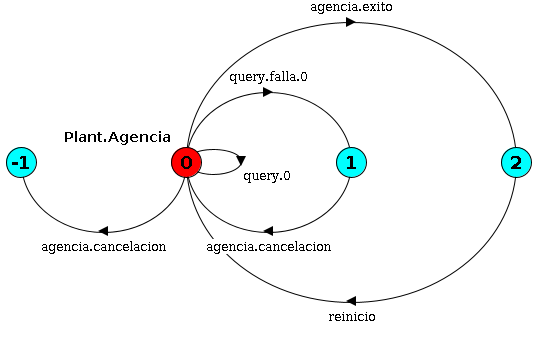
\includegraphics[width=\linewidth]{figures/ejemploServicios/N1Agencia.png}  
				\caption{la agencia}
				\label{fig:agencia}
			\end{subfigure}
			\begin{subfigure}[t]{.6\textwidth}
				\centering
				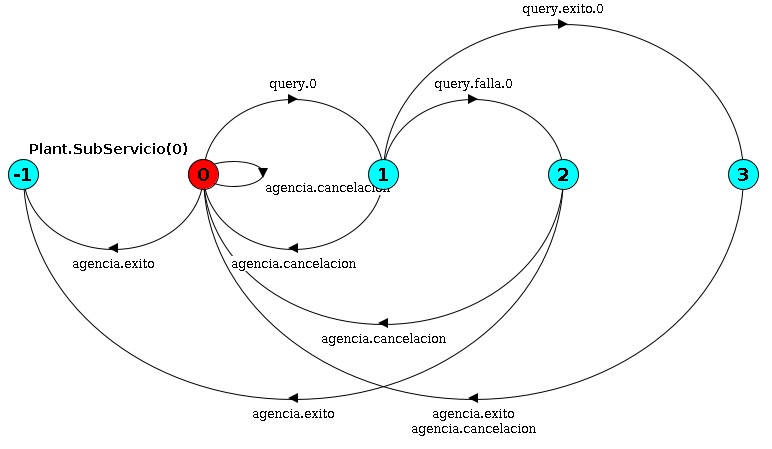
\includegraphics[width=\linewidth]{figures/ejemploServicios/N1SubServicio.png}  
				\caption{el sub servicio a contratar}
				\label{fig:subserv}
			\end{subfigure}
		}
		\makebox[\linewidth][c]{%
			\begin{subfigure}[t]{.6\textwidth}
				\centering
				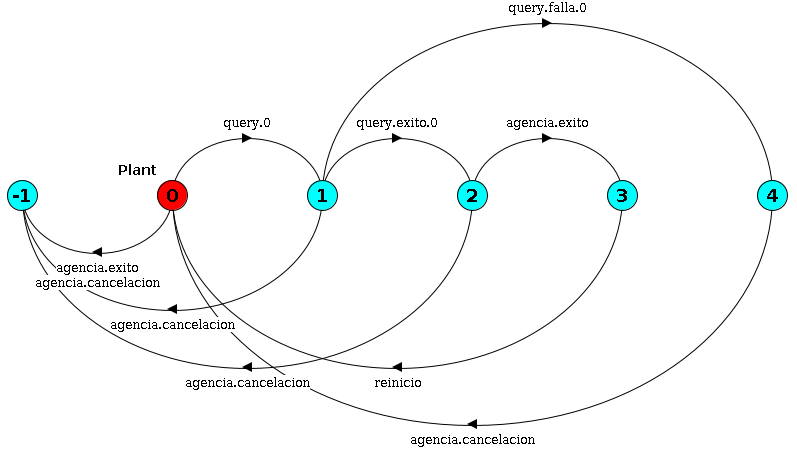
\includegraphics[width=\linewidth]{figures/ejemploServicios/N1Planta.png}  
				\caption{Planta compuesta}
				\label{fig:N1Planta}
			\end{subfigure}
			\begin{subfigure}[t]{.6\textwidth}
				\centering
				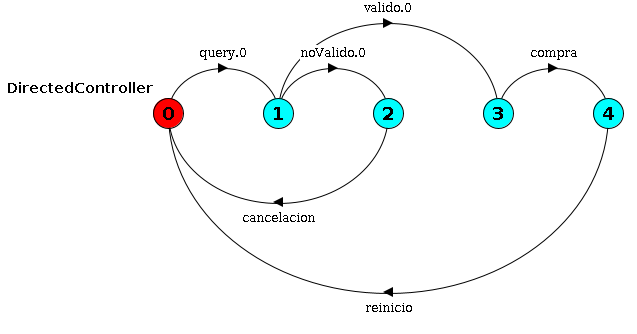
\includegraphics[width=\linewidth]{figures/ejemploServicios/N1Controlador.png}  
				\caption{Controlador resultante}
				\label{fig:controladorN1}
			\end{subfigure}
		}
		\caption{Caso con un solo sub-servicio}
		\label{fig:N1}
	\end{center}
\end{figure}

\begin{figure}[htb]
	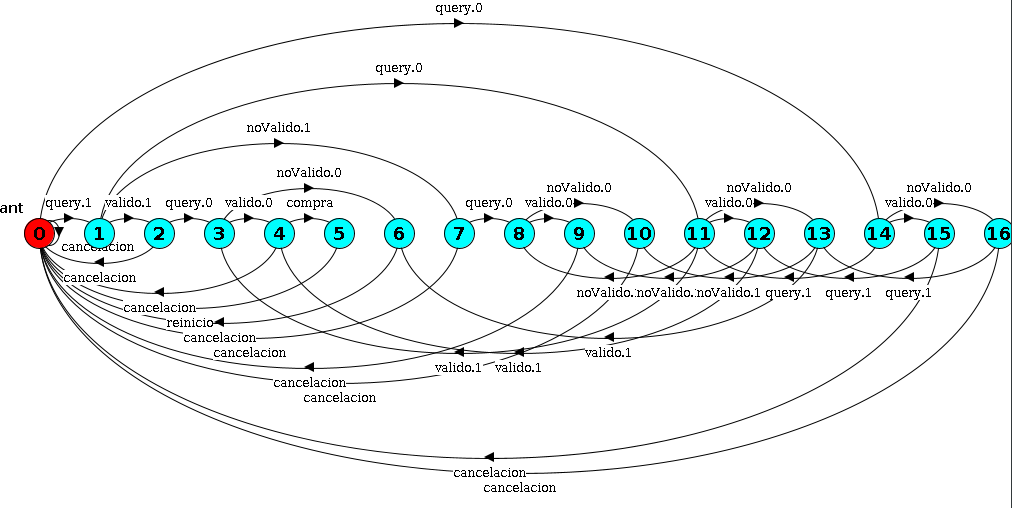
\includegraphics[width=\linewidth]{figures/ejemploServicios/N2Planta.png}  
	\caption{Planta compuesta con 2 sub-servicios}
	\label{fig:N2}
\end{figure}

\begin{figure}[htb]
	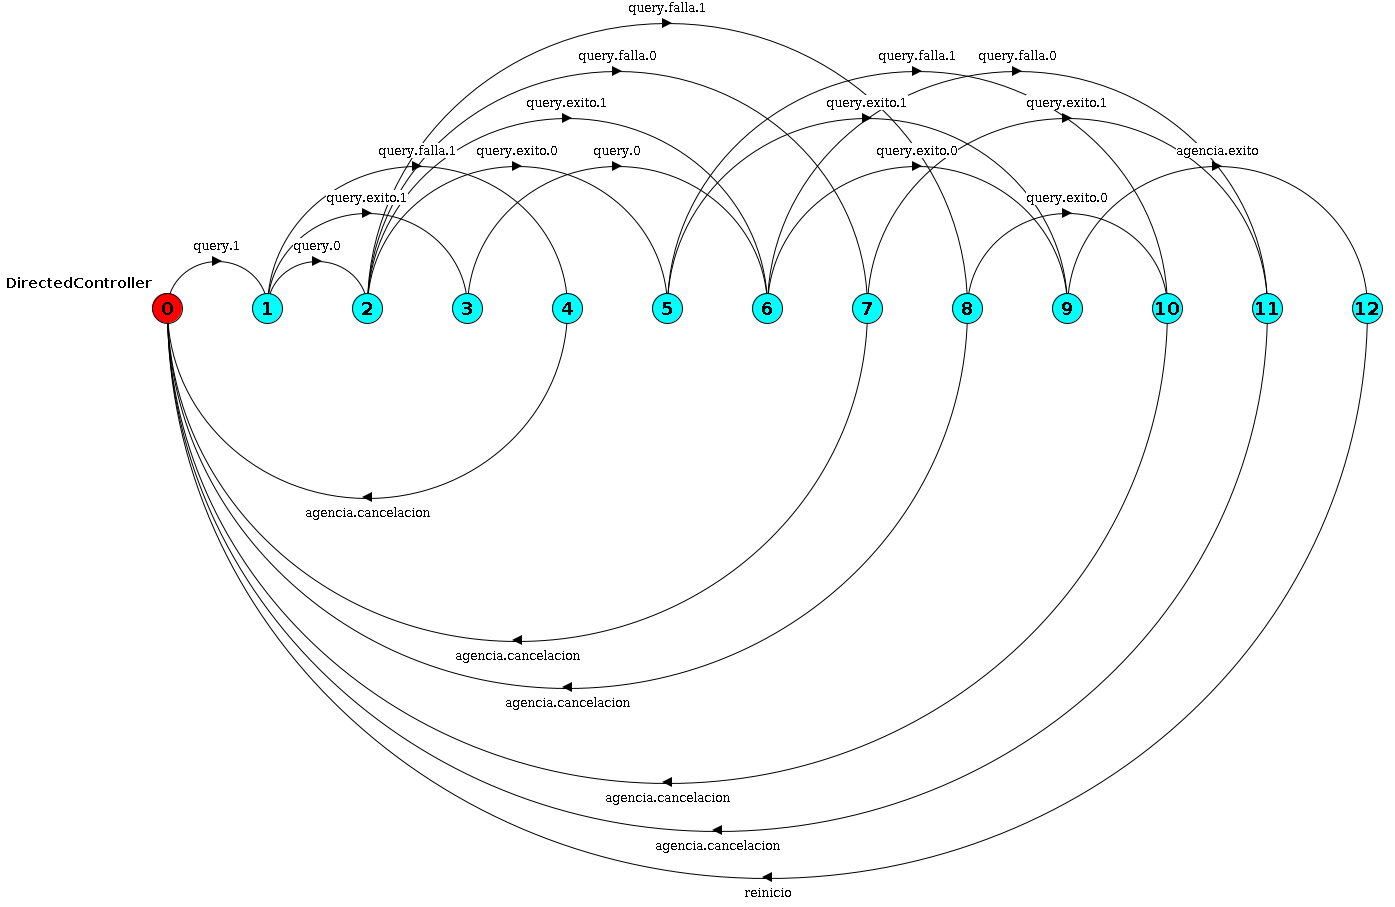
\includegraphics[width=\linewidth]{figures/ejemploServicios/N2Controlador.png}  
	\caption{Controlador para el problema con 2 sub-servicios}
	\label{fig:N2-control}
\end{figure}

En el ejemplo, la figura \ref{fig:agencia} representa a la agencia, que comienza en el estado inicial (0), y lo que quiere es confirmar la compra, el estado 2 es nuestro estado marcado, objetivo que queremos alcanzar infinitas veces. El estado 0 representa un estado en el que no se detectaron problemas con ningún sub-servicio, por lo que permite, cuando los otros componentes se sincronicen, tomar el evento \textit{agencia.exito}. En cambio, al detectar algún \textit{query.falla}, se mueve al estado 1, señalando que hubo un problema y solo permite cancelar la compra de todos los otros servicios consultados.

El componente del subservicio (figura \ref{fig:subserv}) también tiene el evento \textit{agencia.exito}, pero debe previamente haber recibido la consulta (\textit{query.0}) y confirmado su disponibilidad tomando el evento \textit{query.exito.0}. En caso de no ser posible la reserva (\textit{query.falla.0}), solo permite la cancelación de la compra (\textit{agencia.cancelacion}), yendo del estado 2 al 0; si se quisiera confirmar la compra (\textit{agencia.exito}) se llega al estado -1, reservado para los errores que el controlador debe evitar. Además, en caso de que la agencia cancele la compra del paquete de servicios, se vuelve al estado 0 y se espera una consulta.

Recordemos que queremos representar un sistema complejo con interacción de múltiples componentes. Esta sincronización se ve reflejada en la figura \ref{fig:N1Planta}, que muestra la planta que representa al sistema con los dos componentes previamente descriptos. 

Finalmente, \ref{fig:controladorN1} muestra un posible controlador para este problema. Destacamos que todos los eventos controlables que llevaban al estado -1 (el estado error), no son una posibilidad permitida por el controlador. 

Puede verse que para el caso de solo un sub-servicio que debe ser contratado el problema es manejable. Los modelos gráficos de la planta y el controlador, generados automáticamente por MTSA\footnote{Modal Transition System Analyser, \href{https://bitbucket.org/lnahabedian/mtsa/src/master/^}{https://bitbucket.org/lnahabedian/mtsa/src/master/}} se comprenden con un vistazo. Ya el caso con $N=2$ (fig~\ref{fig:N2}) si bien puede generarse una representación gráfica, requiere un trabajo considerable para comprender qué estado del problema representa cada estado del modelo. Simplemente aumentando a $N=5$ ya la planta compuesta cuenta con 1025 estados y 4085 transiciones, imposibilitando mostrarlo en una figura. 

Destacamos del problema con 2 sub-servicios, que el controlador (figura \ref{fig:N2-control}) no solo imposibilita alcanzar el estado error, si no que también reduce las posibilidades en mayor medida. Por ejemplo, en la planta, desde el estado 0, ambos eventos controlables \textit{query.0} y \textit{query.1} son válidos, pero el controlador permite solo \textit{query.1}, esto es acorde a la definición de director (def \ref{def:director}, sección \ref{chpt:director}).

Los algoritmos tradicionales necesitan construir la planta compuesta entera antes de empezar a construir un controlador. Dada la explosión de estados y transiciones evidente en este simple ejemplo, esto resulta muy costoso (a veces imposible), por ende las técnicas del área enfrentan serios inconvenientes al escalar el tamaño de los problemas a resolver. La exploración on-the-fly dirigida busca construir sólo la parte  necesaria de la planta, sacando conclusiones en función de la información obtenida; en el peor caso, termina contruyendo toda la planta y obtiene el controlador de forma tradicional.








